\section{Analyse}
\label{sec:codeanalyse}
Wurden Teile eines Programms programmiert, ist es wichtig dessen Funktion und Leistung zu überprüfen. Neben der Identifikation von Problemen geht es dabei vor allem um Optimierungen. Dieser Abschnitt beschäftigt sich mit automatisierten Verfahren zur Analyse von Software. Zunächst werden die allgemeinen Konzepte statische und dynamische Analyse erklärt. Darauffolgend werden die Vorteile und Grenzen dieser Verfahren erläutert. Abschließend wird ein Werkzeug zur Analyse von Software vorgestellt. 

\subsection{Allgemeine Konzepte}
Die \textbf{statische Quellcodeanalyse} ist ein Verfahren, welches Quellcode unabhängig von der Kompilierung oder Ausführung nach verschiedenen Kriterien auswertet. Dies soll Fehler, Inkonsistenzen und Unsicherheiten im Programmcode aufdecken. Statisch bedeutet in diesem Kontext, dass der Code nicht ausgeführt, jedoch unter anderem auch semantisch ausgewertet wird. Verwendete Verfahren sind \cite[p.~12]{OwaspCodeReview2008}:
\begin{itemize}
	\item[(a)] \textbf {Taint Analyse}: Analyse zur Verhinderung von böswilligen Benutzereingaben, die Code auf dem Hostcomputer ausführen (z.B. SQL Injection)
	\item[(b)] \textbf {Datenfluss Analyse}: Analyse, welche Daten zwischen Programmteilen ausgetauscht werden und welche Abhänigkeiten daraus entstehen.
	\item[(c)] \textbf {Kontrollfluss Analyse}: Analyse zur Evaluation und Integritätsprüfung des Programmablaufes mit dem Ziel der Feststellung von Anomalien (z.B. Endlosschleifen)
	\item[(d)] \textbf {Lexikalische Analyse}: Syntaktische Prüfung des Quellcodes und Generierung von Tokens
\end{itemize}
Historisch ist das Programmierwerkzeug Lint der Pionier der statischen Codeanalyse. Ursprünglich wurde Lint für die Programmiersprache C entwickelt. Nach und nach wurden Abwandlungen für andere Programmiersprachen, darunter beispielsweise JavaScript, TypeScript und Python, entwickelt. Die Entwicklung von Lint lief synergetisch zu der Entwicklung moderner Compiler \cite[p.~2] {Darwin1988}. Ursprünglich sind Lint Programme so gedacht, dass diese vom Benutzer explizit ausgeführt werden müssen und anschließend den Quellcode analysieren.
In modernen IDE sind Lint-ähnliche Verfahren meist automatisch integriert. Diese analysieren kontinuierlich den Quellcode und zeigen mögliche Probleme direkt an (\autoref{fig:lint_vs}). 
Zudem werden solche Analysewerkzeuge als zusätzliche Plugins für viele IDEs angeboten \cite{Darwin1988}\cite{wiki:Lint_Programmierwerkzeug}.

\begin{figure}[!htb] 
	\centering
	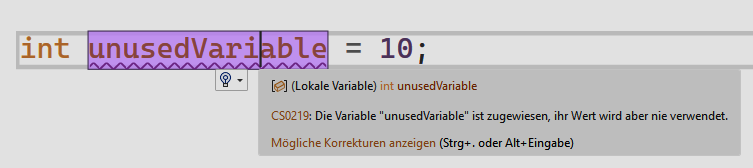
\includegraphics[width=125mm]{images/ide_linting.png}
	\caption{Statische Codeanalyse in Visual Studio}
	\label{fig:lint_vs}
\end{figure}
\FloatBarrier

Die Möglichkeiten der statischen Codeanalyse lassen sich in die Kategorien \textit{Stylechecking}, \textit{Semantische Analyse} und \textit{Weiteres} unterteilen.

\label{subsubsec:style}Bei der Softwareentwicklung wird häufig im voraus ein Programmierstil, auch oft Coding Conventions genannt, festgelegt. Dieser baut auf den üblichen Vorgehensweisen des verwendeten Programmierparadigma auf. Die meisten Programmiersprachen bieten ein Katalog von solchen Codierungsrichtlinien an. So existiert beispielsweise für die objektorientierte Sprache Java ein Dokument mit einer Empfehlung für einen zu verwendenden Programmierstil \cite{java_coding_conventions}.

Für Projekte ist es gegebenenfalls sinnvoll die Codierungsrichtlinien der verwendeten Programmiersprache anzupassen und zu erweitern.
Beispiele für Codierungsrichtlinien sind die Anwendung von Entwurfsmustern, die Festlegung der Namenskonventionen, der Umfang der Dokumentation oder die Gestaltung von Funktionsaufrufen.

Ein \textbf{Style Checker} ist ein Werkzeug, welches die Einhaltung des definierten Programmierstils überprüft. Dies ermöglicht es beispielsweise Verstöße gegen Benennungskonventionen oder einer Überschreitung der maximal zulässigen Zeilenlänge von Code zu erkennen. Style Checker bilden jedoch nur eine Teilmenge davon ab, was mit statischer Codeanalyse möglich ist, da meistens keine semantische Quellcodeanalyse vorgenommen wird.  So kann beispielsweise nicht erklärt werden, dass in \autoref{code:infiniteloop} eine Endlosschleife produziert wurde \cite{lwn.net}\cite{wiki:Style_Checker}.
\begin{lstlisting}[caption={Endlosschleife}, label=code:infiniteloop]
	while (1<10)
	{
	}
\end{lstlisting}
\FloatBarrier
In der \textbf{semantischen Analyse} wird der Quellcode auf inhaltliche Konsistenz und mögliche Fehler geprüft. So können beispielsweise folgende Probleme erkannt werden: Memory Leaks, Pufferüberläufe, Divisionen durch null, Array Zugriffe außerhalb der Grenzen, Endlosschleifen, mögliche Nullverweise, nicht verwendete Variablen und Methoden, Anti-Patterns, mögliche Code Injections, Substitutionen und Generalisierungen oder toter Quellcode. Diese Art der Analyse ist besonders wichtig, da sie folgenschwere Fehler aufdecken soll.

Wird ein objektorientiertes Programmierparadigma verwendet besteht eine \textbf{weitere Möglichkeit} in der Bestrebung durch statische Quellcodeanalysen das Design zu bewerten. Dies ist natürlich nicht vollumfänglich möglich, jedoch gibt es bestimmte statisch ermittelbare Metriken, die 
auf ein gutes oder schlechtes Design schließen lassen. Diese lassen sich aus den Prinzipien für ein agiles, objektorientiertes Design ableiten \cite{Martin2002-nf}. Folgende Metricken sind hierfür denkbar und teilweise auch schon in statischen Analysewerkzeugen implementiert \cite{OwaspCodeReview2008}\cite{Darwin1988}\cite{jetbrains_static_analyse}\cite{wiki:Statische_Code-Analyse}:
\begin{itemize}
	\item[(a)] Lines of Code (Single Responsiblility)
	\begin{itemize}
		\item Innerhalb einer Komponente, Komponente oder Methode
	\end{itemize}	
	\item[(b)] Ringabhänigkeiten
	\item[(c)] Coderedundanzen (Don't repeat yourself, Abstraction)
	\item[(d)] Große Vererbungsstrukturen (Composition over inheritance)
	\item[(e)] Abhänigkeiten auf Implementierungen statt auf Interfaces (Dependency Inversion, Open-Closed)
	\item[(f)] Größe der Interfaces (Interface Seggregation)
	\item[(g)] Fehlende Implementierungen für Basismethoden (Liskov Subsitution)
\end{itemize}

Bei der \textbf{dynamischen Analyse} liegt der Fokus auf Bereichen, die nicht von der statischen Quellcodeanalyse abgedeckt werden können. Dies sind primär Fehler in der Anwendungslogik, fehlende Sicherheitsvalidierung und Performance. 

Wesentlich wird die dynamische Analyse von sogenannten Profiling Werkzeugen abgewickelt. Diese können verschiedene Messwerte zu der entwickelten Software ermitteln. Dazu gehört die Anzahl der Funktionsaufrufe und Funktionsdurchläufe, die Speicherauslastung, nicht freigegebenen Speicherbereiche, nebenläufige Prozesse und Deadlocks. Durch statistische Analysen kann herausgefunden werden, welche Programmteile lohnenswert optimierbar sind, um eine bessere Leistungs- und Speicherperformance zu erhalten. Auch Fehler in der Anwendungslogik, die sich in Deadlocks oder Memoryleaks manifestieren, können aufgedeckt werden \cite{mci/Papenbrock2019}\cite{wiki:Profiler_Programmierung}\cite{computerweekly_dynamic_code}\cite{embedded_swe_codeanalysis}. \label{subsubsec:dynamic}


\subsection{Vorteile und Grenzen}
\label{subsec:Codeanalyse_risks}
Durch Automatisierte Analyseverfahren können tausende Zeilen Quellcode in kürzester Zeit mit einer sehr hohen Präzision durchsucht und ausgewertet werden. Mögliche Problemstellen werden unmittelbar angezeigt und können meist auch zur Quelle zurückverfolgt werden (z.B. nicht validierte Parameter). Über Konfigurationen können die Codeconventions festgelegt werden und Antipatterns definiert werden, die anschließend bei der statischen Codeanalyse überprüft werden. So kann auch in großen Projekten eine Einheitlichkeit und Stabilität im Quellcode erreicht und somit die Softwarequalität erhöht werden.
Häufig auftretende Probleme oder Muster, die zu Schwierigkeiten im Entwicklungsprozess führen können, sind in den Analysewerkzeugen bereits vorkonfiguriert.
Intellegente Analysewerkzeuge bieten zudem die Möglichkeit einer automatischen Problembehebung. Hier wird der Quellcode automatisch refaktorisiert (\autoref{sec:refactor}) oder abgeändert.

Auch wenn Analysewerkzeuge eine große Hilfe für Softwareentwickler darstellen, ist es wichtig die Grenzen dieser zu kennen. Analysewerkzeuge sind nur so gut, wie sie programmiert und konfiguriert wurden. Sind bestimmte Antipatterns oder Konstrukte für unsauberen Code nicht in der Konfiguration und Programmierung berücksichtigt, werden diese auch nicht erkannt. Zudem lassen sich auch technisch nicht alle Problemfelder ermitteln. So können Logikfehler in komplexen Geschäftsprozessen häufig nicht identifiziert werden, da das Analysewerkzeug kein Verständnis hierfür besitzt. Auch bei Framework-spezifischen Anwendungsfeldern können Probleme auftreten, da die Analysewerkzeuge auf die Framework Version abgestimmt sein müssen. Werden spezielle Techniken verwendet, wie z.B. Dependency Injection, die bei der Implementierung des Werkzeuges nicht berücksichtigt sind, kann es ebenfalls zu Schwierigkeiten kommen. So kann es in diesem Fall sein, dass Abhängigkeiten nicht mehr nachvollzogen werden können, weil keine klassische Referenzerzeugung und Übergabe mehr stattfindet. Sprachen die ständig weiter entwickelt werden, erzwingen ebenfalls eine kontinuierliche Weiterentwicklung der zugehörigen Analysewerkzeuge \cite{OwaspCodeReview2008}\cite{wiki:Statische_Code-Analyse}\cite{embedded_swe_codeanalysis}. 

\subsection{Beispiel Werkzeug}
\label{subsec:Codeanalyse_analyse}
Als eine Suite von Beispielwerkzeugen werden die Produkte des Softwareherstellers JetBrains gewählt. Die Werkzeuge sind entweder in die IDEs, die von Jetbrains angeboten werden integriert, oder als seperates Plugin für Visual Studio oder den Standalonebetrieb verfügbar. Angeboten werden:
\begin{itemize}
	\item[(a)] ReSharper (Statische Codeanalyse, Refactoring)
	\item[(b)] DotTrace (Dynamische Analyse, Leistungsprofiling)
	\item[(c)] DotMemory (Dynamische Analyse, Memoryprofiling)
	\item[(d)] DotCover (Statische und dynamische Analyse, Testabdeckung, Unittesting)
\end{itemize}
Jetbrains bietet elf IDEs für verschiedene Programmiersprachen an, die alle auf einem gemeinsamen Framework basieren \cite{intelliJPlattform}. Somit werden die Sprachen Objective C, Swift, PHP, Python, C\#, Visual Basic, Go, Rust, Ruby, Kotlin, JavaScript und Java unterstützt \cite{jetbrains_products}. 
%https://faculty.sist.shanghaitech.edu.cn/faculty/songfu/cav/PPA.pdf
%Artificial Intelligence Methods For Software Engineerin
%https://de.wikipedia.org/wiki/Statische_Code-Analyse
%https://www.techtarget.com/searchsoftwarequality/news/252523049/Developers-beware-AI-pair-programming-comes-with-pitfalls
%https://dl.acm.org/doi/pdf/10.1145/318774.318944
%file:///D:/Users/Jona/Downloads/ESSCAT-report-for-printing-1.pdf